\documentclass[12pt]{exam}
\usepackage[utf8]{inputenc}
\usepackage{graphicx} % Allows including images
\usepackage{cool}
\usepackage{tikz}
\usepackage{amsmath}
\usepackage{listings}
\usepackage[colorlinks = true,
            linkcolor = blue,
            urlcolor  = blue,
            citecolor = blue,
            anchorcolor = blue]{hyperref}
\usepackage{pseudocode}
\usepackage{MnSymbol,wasysym}
\usepackage{geometry} % see geometry.pdf on how to lay out the page. There's lots.
\geometry{a4paper} 
\newgeometry{vmargin={20mm}, hmargin={14mm,18mm}}
 
\begin{document}
\begin{center}
{\large {\bf Stanford CME 241 (Winter 2020) - Final Exam Solutions}}

\end{center}
\vspace{5mm}
 
\begin{questions}
\question{\bf Optimal Croaking on Lilypads} Consider an array of $n+1$ lilypads on a pond, numbered $0$ to $n$. A frog sits on a lilypad other than the lilypad numbered $0$ or $n$.  When on lilypads $i$ ($1\leq i \leq n-1$), the frog can croak one of two sounds $A$ or
$B$. If it croaks $A$ when on lilypad $i$ ($1 \leq i \leq n-1$), it is thrown to lilypad $i-1$ with probability $\frac i n$ and is thrown to lilypad $i+1$ with probability $\frac {n-i} n$. If it croaks $B$ when on lilypad $i$ ($1\leq i \leq n-1$), it is thrown to one of the lilypads $0, \ldots, i-1, i+1, \ldots n$ with uniform probability $\frac 1 n$. A snake, perched on lilypad $0$, will eat the frog if the frog lands on lilypad $0$. The frog can escape the pond (and hence, escape the snake!) if it lands on lilypad $n$.

What should the frog croak when on each of the lilypads $1, 2, \ldots, n-1$, in order to maximize the probability of escaping the pond (i.e., reaching lilypad $n$ before reaching lilypad $0$)? Although there are more than one ways of solving this problem, we'd like to solve it by modeling it as an MDP and identifying the Optimal Policy.

\begin{itemize}
\item {\bf 3 points:} Express with clear mathematical notation the state space, action space, transitions function and rewards function of an MDP so that the above {\em frog-escape} problem is solved by arriving at the Optimal Value Function (and hence, the Optimal Policy) of this MDP.

{\bf Answer: } The state space $\mathcal{S} = \{i \mid 0 \leq i \leq n\}$, with each state $i$ representing the number of the lilypad the frog is on. States $i=0$ and $i=n$ are terminating states. The action space $\mathcal{A} = \{A,B\}$ corresponding to the two choices of croak sounds. The state transitions are given by:
$$
Pr[i' \mid (i,A)]  \text{ for } 1 \leq i \leq n-1 =
\begin{cases}
\frac i n & \text{ for } i' = i - 1\\
\frac {n-1} n  & \text{ for } i' = i + 1\\
0 & \text{ otherwise}
\end{cases}
$$
$$
Pr[i' \mid (i,B)]  \text{ for } 1 \leq i \leq n-1 =
\begin{cases}
 \frac 1 n & \text{ for all } 0 \leq i' \leq n \text{ and } i' \neq i\\
 0 & \text{for } i' = i
 \end{cases}
$$
Let us define $R(i, a, i')$ as the {\em Reward} when transitioning to state $i'$ from state $i$ upon taking action $a$.
$$
R(i, a, i') \text{ for } 1\leq i \leq n-1, a \in \{A,B\} = 
\begin{cases}
1 & \text{ for } i' = n\\
0 & \text{ otherwise}
\end{cases}
$$

\item {\bf 6 points:} Write working Python code (with type annotations and comments) that models this MDP and solves the Optimal Value Function and Optimal Policy (you can re-use any code you have written previously as part of this course's suggested assignments). Remember to include your Python code in your answer submission.

{\bf Answer:} The Python code that models this MDP and solves the Optimal Value Function and Optimal Policy is \href{https://github.com/coverdrive/MDP-DP-RL/blob/master/src/examples/exam_problems/frog_lilypad.py}{here}.

\item {\bf 3 points:} Using your code, plot a graph of the Optimal Escape-Probability and of the associated Optimal Croak, as a function of the states of this MDP, for $n=3, n=10$ and $n=25$. Include these graphs in your answer submission. By looking at the results on this graph, what pattern do you observe for the optimal policy as you vary $n$ from 3 to 25? 

{\bf Answer:} Running the code for $n=3, n=10, n=25$ gives the following graphs for the Optimal Action-Value Function ($Q^*$) and hence, we can read off the Optimal State-Value Function and the Optimal Policy from these graphs for the respective cases of $n=3, n=10, n=25$. The pattern we observe for the Optimal Policy as we vary $n$ is that for $i=1$, the Optimal Action is Croak $B$ and for $2 \leq i \leq n-1$, the optimal action is Croak $A$.

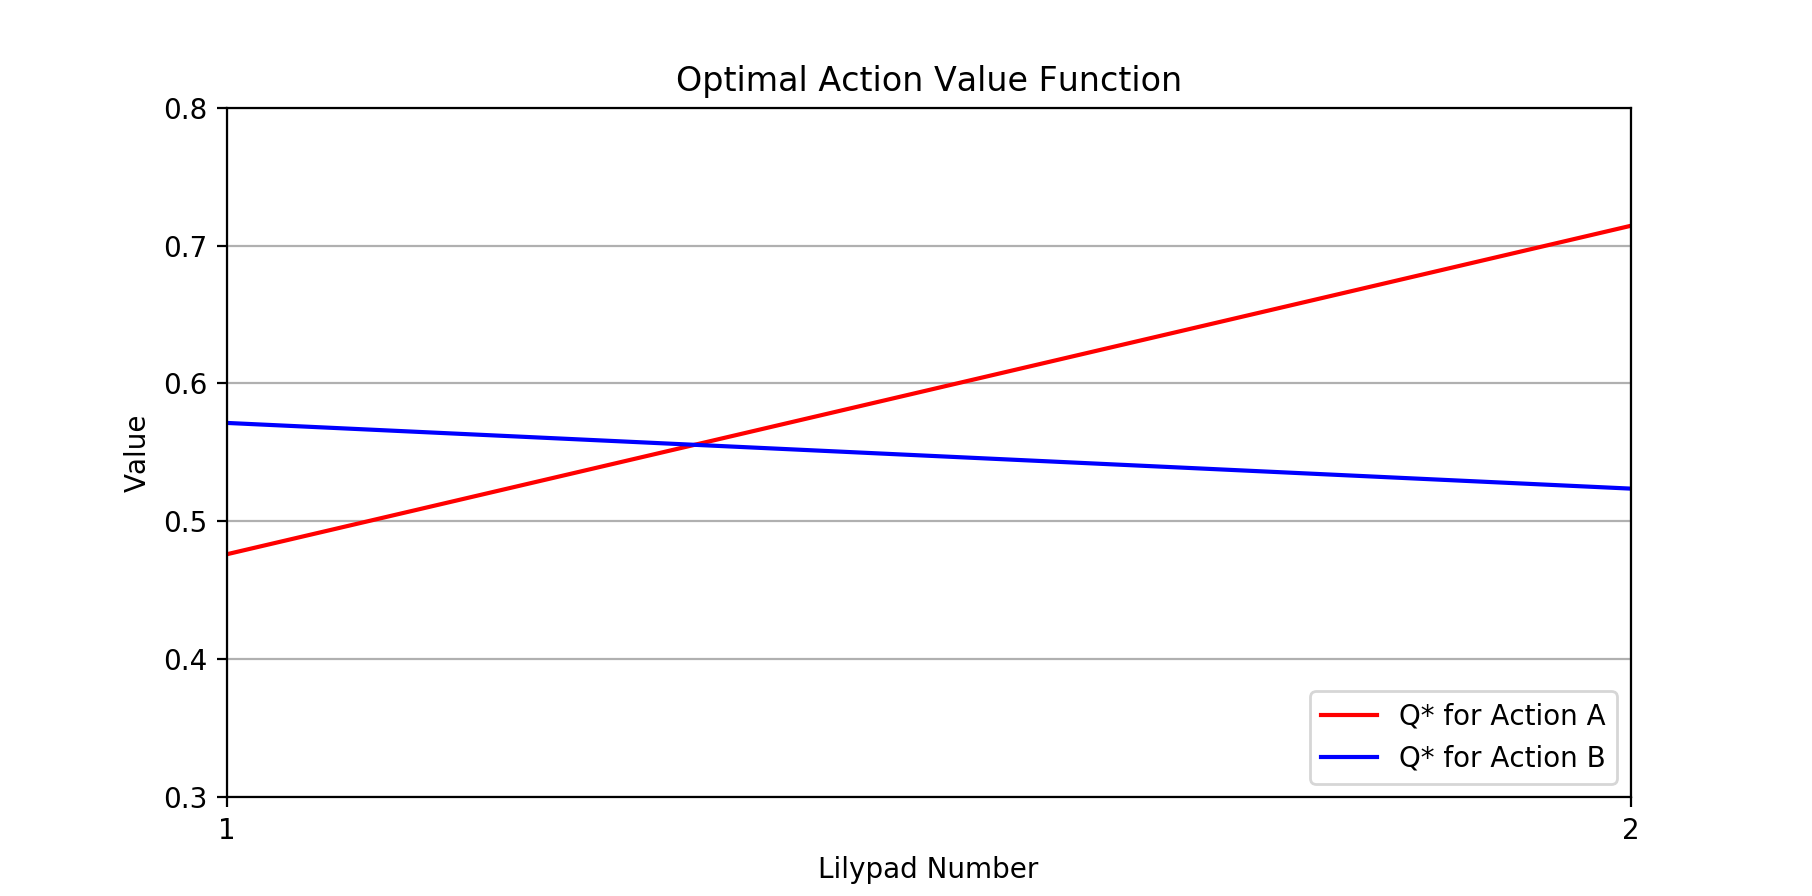
\includegraphics[width=18cm, height=6cm]{lilypad3.png}

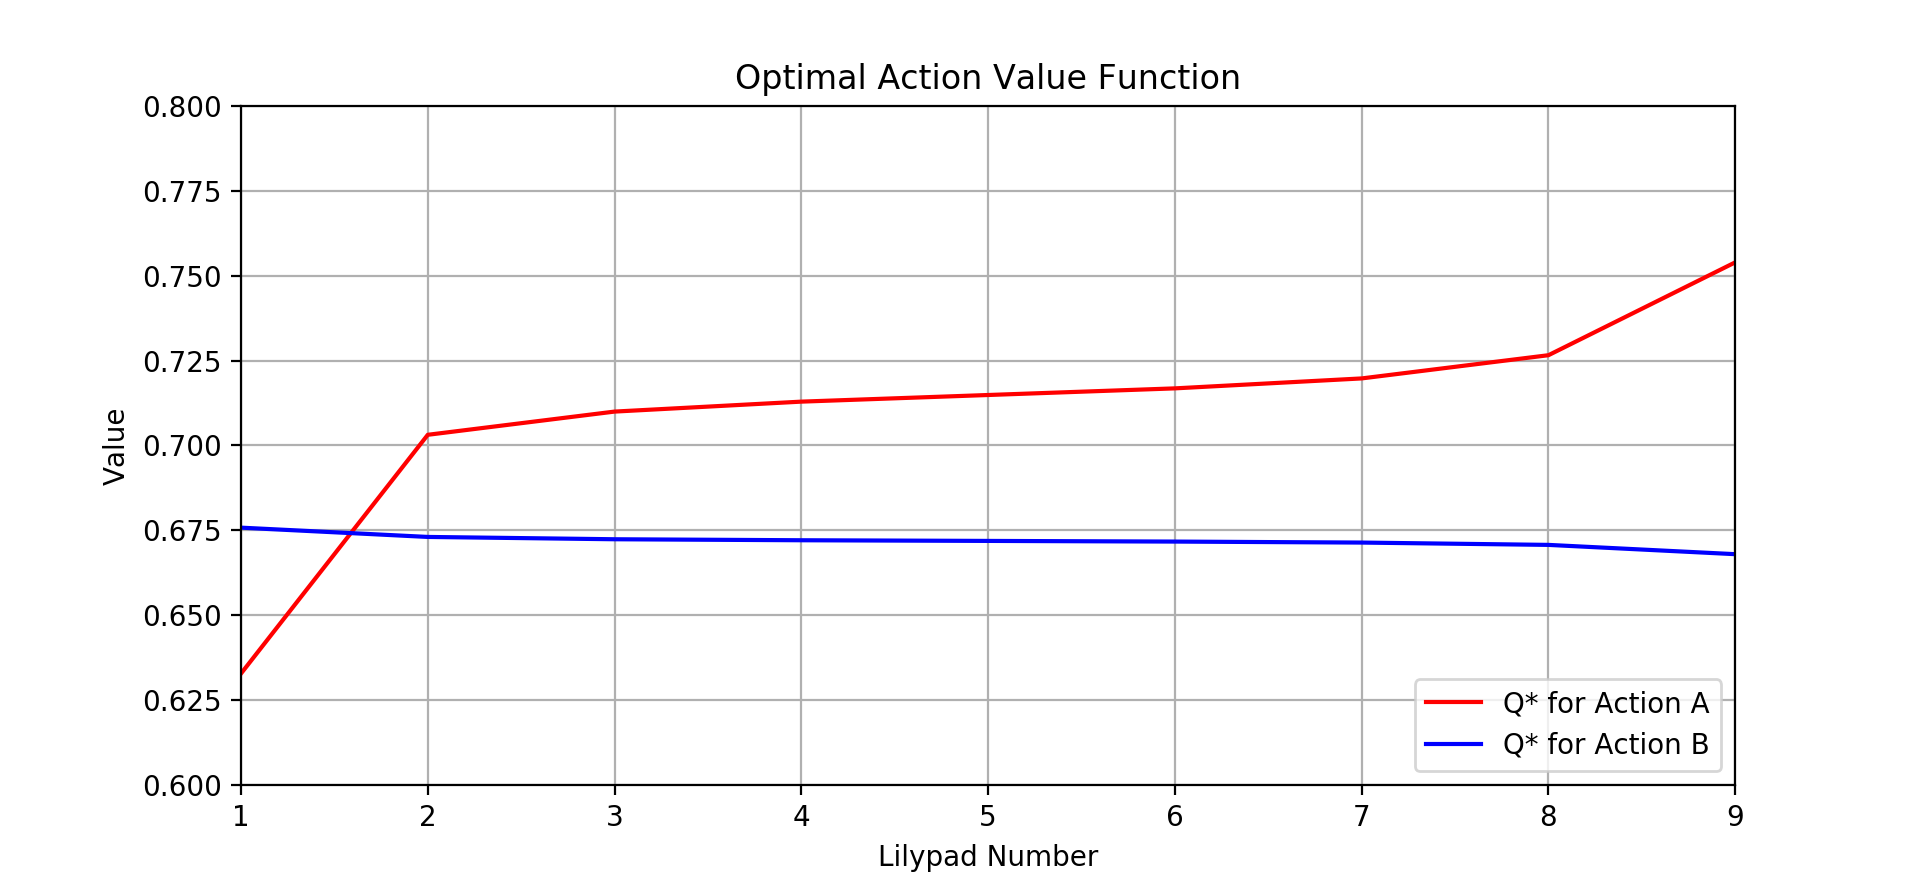
\includegraphics[width=18cm, height=6cm]{lilypad10.png}

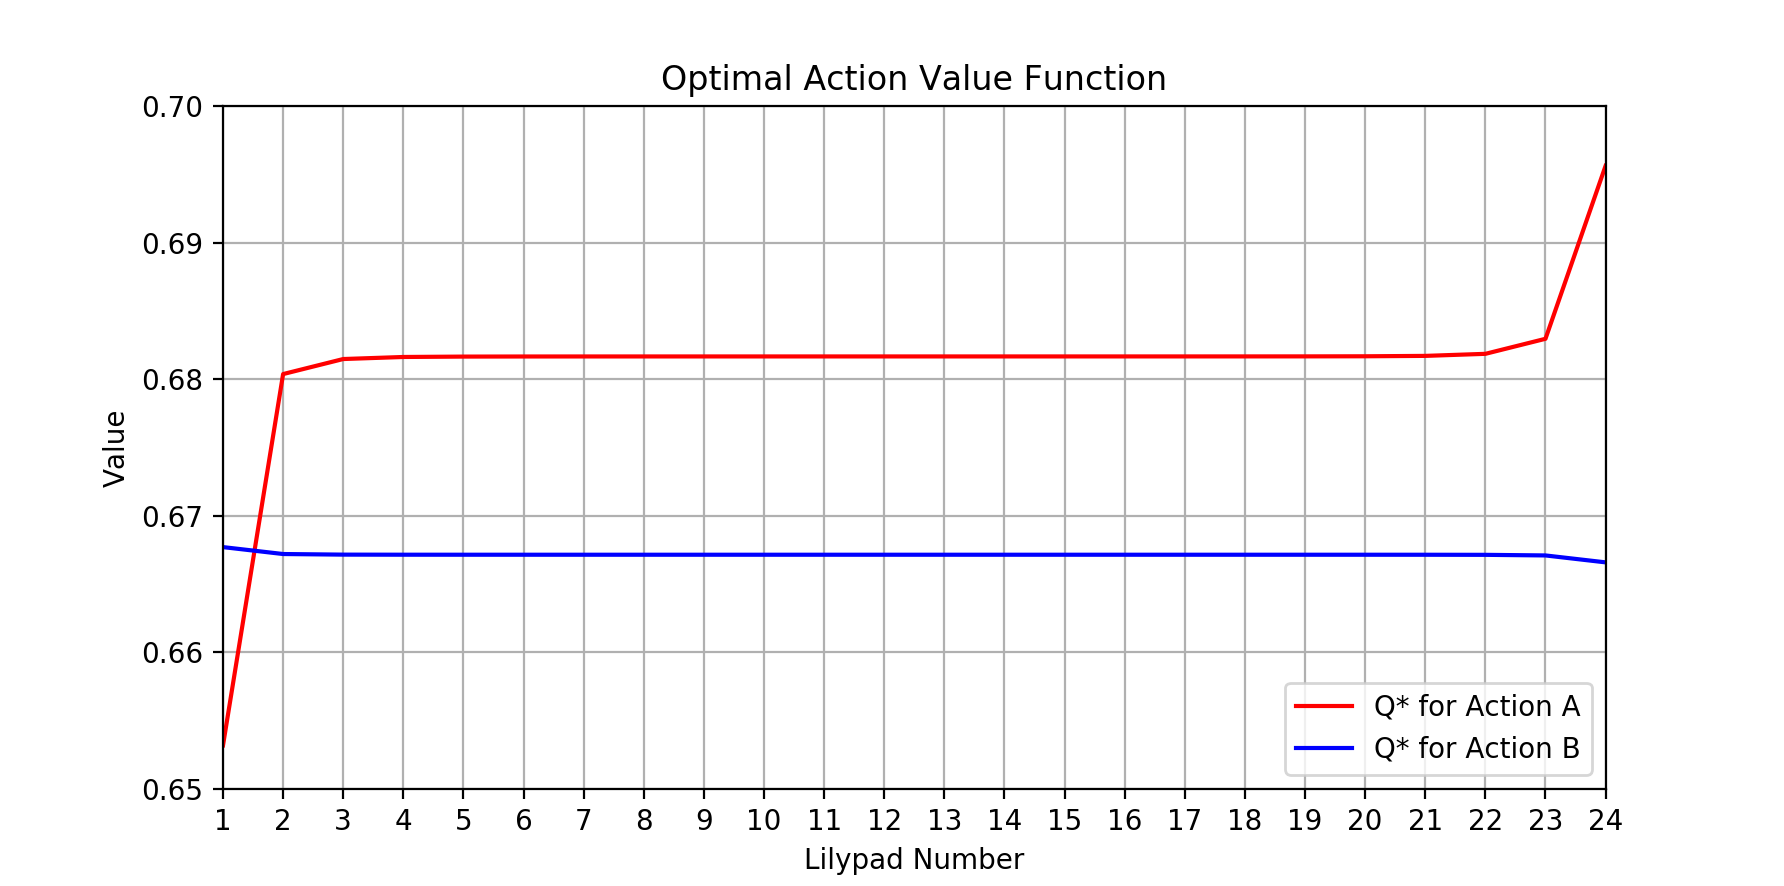
\includegraphics[width=18cm, height=6cm]{lilypad25.png}


\end{itemize}

\vspace{3mm}
\question{\bf Job-Hopping and Wage-Maximization}. You are a worker who starts every day either employed or unemployed. If you start your day employed, you work on your job for the day (one of $n$ jobs, as elaborated later) and you get to earn the wage of the job for the day. However, at the end of the day, you could lose your job with probability $\alpha \in [0,1]$, in which case you start the next day unemployed. If at the end of the day, you do not lose your job (with probability $1-\alpha$), then you will start the next day with the same job (and hence, the same daily wage). On the other hand, if you start your day unemployed, then you will be randomly offered one of $n$ jobs with daily wages $w_1, w_2, \ldots w_n \in \mathbb{R}^+$ with respective job-offer probabilities $p_1, p_2, \ldots p_n \in [0,1]$ (with $\sum_{i=1}^n p_i = 1$). You can choose to either accept or decline the offered job. If you accept the job-offer, your day progresses exactly like the {\em employed-day} described above ((earning the day's job wage and possibly (with probability $\alpha$) losing the job at the end of the day). However, if you decline the job-offer, you spend the day unemployed, receive the unemployment wage $w_0 \in \mathbb{R}^+$ for the day, and start the next day unemployed. The problem is to identify the optimal choice of accepting or rejecting any of the job-offers the worker receives, in a manner that maximizes the infinite-horizon {\em Expected Discounted-Sum of Wages Utility}. Assume the daily discount factor for wages (employed or unemployed) is $\gamma \in [0,1)$. Assume CRRA utility function $U(w) = \frac {w^{1-a} - 1} {1-a}$ for CRRA risk-aversion parameter $a \in \mathbb{R}$ (for $a=1$, $U(w) = \log w$). So you are looking to maximize
$$\mathbb{E}[\sum_{u=t}^\infty \gamma^{u-t} \cdot U(w_{i_u})]$$
 at the start of a given day $t$ ($w_{i_u}$ is the wage earned on day $u$, $0\leq i_u \leq n$ for all $u\geq t$).

\begin{itemize}
\item {\bf 5 points}: Express with clear mathematical notation the state space, action space, transition function, reward function, and write the Bellman Optimality Equation customized for this MDP.

{\bf Answer: } We denote the state space as $\mathcal{S} = \{i \mid 1 \leq i \leq n\} \times \{E, U\}$. So the state is represented by an (int, str) pair where the str (U or E) denotes being unemployed or employed and the int ($1\leq i \leq n$) denotes the index of the job employed in (if E) or the job offered (if U). The possible actions are $a=A$ (``accept the job-offer'') or $a=D$ (``decline the job-offer''). However, we need to choose between accepting or declining the job-offer only in unemployed states. Therefore, we structure the action space as a function of the state as follows: $\mathcal{A}((i, U)) = \{A,D\}$ for all $1\leq i \leq n$ and $\mathcal{A}((i, E)) = \{A\}$ for all $1 \leq i \leq n$ (to indicate that we don't need to make any choice when employed).

For all $1\leq i \leq n$, the state transitions are as follows:
$$
Pr[(i',b') \mid (i,b), A] =
\begin{cases}
\alpha \cdot p_{i'} & \text{ for each } 1 \leq i' \leq n, \text{for each } b \in \{U,E\}, \text{and } b' = U\\
1 - \alpha & \text{ for } i' = i, \text{for each } b \in \{U, E\}, \text{and } b' = E\\
0 & \text{ otherwise}
\end{cases}
$$
$$
Pr[(i',b') \mid (i,U), D] =
\begin{cases}
p_{i'} & \text{ for each } 1 \leq i' \leq n, \text{and } b' = U\\
0 & \text{ otherwise}
\end{cases}
$$

Let us define $R((i,b), a)$ as the {\em Expected Reward} obtained when in state $(i,b)$ upon taking action $a$.
$$R((i,b),A) = U(w_i) \text{ for each } 1\leq i\leq n, \text{for each } b \in \{U,E\}$$
$$R((i,U),D) = U(w_0) \text{ for each } 1\leq i\leq n$$

The Bellman Optimality Equation for the Optimal Value Function $V^* : \mathcal{S} \rightarrow \mathbb{R}$ is as follows:

For all $1\leq i \leq n$

$$V^*((i,U)) = \max(U(w_0) + \gamma \cdot \sum_{i'=1}^n p_{i'} \cdot V^*((i', U)), V^*((i,E))) $$
$$V^*((i,E)) = U(w_i) + \gamma (\alpha \cdot \sum_{i'=1}^n p_{i'} \cdot V^*((i', U)) + (1 - \alpha) \cdot V^*((i,E)) ) $$

We can simplify the above by denoting $\sum_{i'=1}^n p_{i'} \cdot V^*((i', U))$ as $V_0$ and $V^*((i,E))$ as $V_i$ for all $1\leq i \leq n$. This yields:

$$V_0 = \sum_{i'=1}^n p_{i'} \cdot \max(U(w_0) + \gamma \cdot V_0, V_{i'})$$
$$V_i = U(w_i) + \gamma \cdot (\alpha \cdot V_0 + (1 - \alpha) \cdot V_i) \text{ for all } 1 \leq i \leq n$$
This is the more succinct (and easy-to-implement) version of the Bellman Optimality Equation (in $V_i, 0 \leq i \leq n$).
Hence, one would accept job-offer $i$ (for $1 \leq i \leq n$) if and only if:
$$V_i > U(w_0) + \gamma \cdot V_0$$

\item {\bf 3 points}: You can solve this Bellman Optimality Equation (hence, solve for the Optimal Value Function and the Optimal Policy) with a numerical iterative algorithm (essentially a Dynamic Programming algorithm customized to this problem). Write Python code for this numerical algorithm. Clearly define the inputs and outputs of your algorithm with their types (int, float, List, Mapping etc.). Remember to include your Python code in your answer submission. Unlike the previous problem, here I am not expecting working Python code - a sketch of Python code that illustrates the numerical algorithm suffices for this problem (however, I need Python syntax so I can understand your approach).

{\bf Answer:} The Python code with the numerical algorithm that solves the above Bellman Optimality Equation (in $V_i, 0 \leq i \leq n$) is \href{https://github.com/coverdrive/MDP-DP-RL/blob/master/src/examples/exam_problems/wage_max.py}{here}.

\end{itemize}

\question {\bf Solving a continuous states/actions MDP analytically}. {\bf 5 points:} Consider a continuous-states, continuous-actions, discrete-time, infinite-horizon MDP with state space as $\mathbb{R}$ and action space as $\mathbb{R}$. When in state $s\in \mathbb{R}$, upon taking action $a\in \mathbb{R}$, one transitions to next state $s' \in \mathbb{R}$ according to a normal distribution $s' \sim \mathcal{N}(s, \sigma^2)$ for a fixed variance $\sigma^2 \in \mathbb{R}^+$. The corresponding cost associated with this transition is $e^{as'}$, i.e., the cost depends on the action $a$ and the state $s'$ one transitions to. The problem is to minimize the  infinite-horizon {\em Expected Discounted-Sum of Costs} (with discount factor $\gamma$). For the purpose of this exam, solve this problem just for the special case of $\gamma = 0$ (i.e., the myopic case) using elementary calculus. Derive an analytic expression for the optimal action in any state and the corresponding optimal cost.

{\bf Answer: } The optimal value function is given by:
\begin{align*}
V^*(s) & = \max_{a \in \mathbb{R}} \{ \mathbb{E}_{s' \sim \mathcal{N}(s,\sigma^2)}[-e^{as'}] \}\\
& = \max_{a \in \mathbb{R}} \{ \int_{-\infty}^{+\infty} \frac {-1} {\sqrt{2\pi} \sigma} \cdot e^{-\frac {(x - s)^2} {2\sigma^2}} \cdot e^{ax} \cdot dx \} \\
& = \max_{a \in \mathbb{R}}  \{ \int_{-\infty}^{+\infty} \frac {-1} {\sqrt{2\pi} \sigma} \cdot e^{-\frac {(x-(s +a\sigma^2))^2} {2\sigma^2}} \cdot e^{s a + \frac {\sigma^2 a^2} {2}} \cdot dx \}\\
& = \max_{a \in \mathbb{R}} \{-e^{s a + \frac {\sigma^2 a^2} 2} \cdot \int_{-\infty}^{+\infty} \frac {1} {\sqrt{2\pi} \sigma} \cdot e^{-\frac {(x-(s +a\sigma^2))^2} {2\sigma^2}} \cdot dx \} \\
& = \max_{a \in \mathbb{R}} \{-e^{s a + \frac {\sigma^2 a^2} 2} \cdot \mathbb{E}_{x\sim \mathcal{N}(s + a\sigma^2, \sigma^2)}[1] \} \\
& = \max_{a \in \mathbb{R}} \{ -e^{s a + \frac {\sigma^2 a^2} 2} \}
\end{align*}
We identify the optimal action $a^*$ that maximizes $-e^{s a + \frac {\sigma^2 a^2} 2}$ as follows:

$$\pderiv{\{-e^{s a + \frac {\sigma^2 a^2} 2}\}}{a} = 0$$
$$ \Rightarrow s + a^* \sigma^2 = 0$$
$$\Rightarrow a^* = \frac {-s} {\sigma^2}$$
We also note that: $$\pderiv[2]{\{-e^{s a + \frac {\sigma^2 a^2} 2}\}}{a} < 0 \mbox{ for } a = a^* = \frac {-s} {\sigma^2}$$

So, $a = a^* = \frac {-s} {\sigma^2}$ maximizes $-e^{s a + \frac {\sigma^2 a^2} 2}$.

Substituting $a^*$ in $ -e^{s a + \frac {\sigma^2 a^2} 2}$, we get:
$$V^*(s) =  -e^{s a^* + \frac {\sigma^2 {a^*}^2} 2} = -e^{-\frac {s^2} {2 \sigma^2}}$$

Therefore, the optimal action in state $s$ is $\frac {-s} {\sigma^2}$ and the corresponding optimal cost is $e^{-\frac {s^2} {2 \sigma^2}}$

 
\end{questions}

\end{document}